% Chapter 5: Kết quả thực nghiệm
\chapter{Kết quả thực nghiệm}

Chương này trình bày kết quả kiểm chứng phần cứng và phần mềm của \textbf{FC-v01} trên bệ thử tĩnh -- giai đoạn trước khi tích hợp thành bộ điều khiển bay hoàn chỉnh và bay ngoài trời. Toàn bộ số liệu trong chương là dữ liệu đo thật, thu qua ba kênh: bộ ghi dữ liệu bay (blackbox) lưu lên thẻ microSD, bộ ghi định thời (trace profiler -- công cụ ghi lại thời điểm bắt đầu và kết thúc của từng vòng làm việc của mỗi tác vụ) và bản tin chẩn đoán qua cổng nối tiếp. Mục~\ref{sec:kq-moitruong} mô tả môi trường thử nghiệm, mục~\ref{sec:kq-cambien} đánh giá chất lượng tín hiệu cảm biến, mục~\ref{sec:kq-ekf} kiểm chứng khối ước lượng, mục~\ref{sec:kq-rtos} đo hiệu năng bộ định thời, mục~\ref{sec:kq-tonghop} tổng hợp các kết quả.

\section{Môi trường và phương pháp thử nghiệm}\label{sec:kq-moitruong}

Mọi thí nghiệm thực hiện trên bệ thử tĩnh: bản mạch v2 đặt cố định trên mặt bàn, không gắn động cơ, cấp nguồn qua cổng USB. Ở điều kiện này, tín hiệu cảm biến phản ánh đúng nhiễu của chính cảm biến và mạch điện, chưa trộn thêm rung động của động cơ -- yếu tố chỉ xuất hiện khi bay thật.

Phần mềm thu dữ liệu ở một trong hai chế độ ghi thẻ, hai chế độ này loại nhau vì cùng dùng thẻ SD. Chế độ thứ nhất, blackbox, ghi sáu luồng cảm biến -- thô và đã lọc của gia tốc kế, con quay hồi tiếp, từ kế -- cùng áp suất, với tần số 500, 100 và 50~Hz. Chế độ thứ hai, trace, ghi thời điểm thực thi của toàn bộ 19 tác vụ. Trước mỗi phiên đo, hệ thống tự chạy một loạt năm cổng kiểm tra tự động (bảng~\ref{tab:kq-gates}); phiên đo chỉ được bắt đầu khi cả năm cổng đều đạt, bảo đảm dữ liệu thu về đến từ hệ thống đứng yên, dữ liệu tươi và đã hiệu chuẩn.

\begin{table}[h]
\centering
\caption{Năm cổng kiểm tra tự động trước mỗi phiên đo}
\label{tab:kq-gates}
\begin{tabular}{p{1.1cm}p{6.2cm}p{7.2cm}}
\toprule
Cổng & Kiểm tra & Tiêu chí đạt \\
\midrule
1 & Dữ liệu luồng cảm biến & Đủ dữ liệu, độ tươi: con quay/gia tốc kế dưới 50~ms, từ kế dưới 100~ms, áp suất dưới 200~ms; giá trị nằm trong khoảng hợp lý \\
2 & Đứng yên & Biến thiên con quay dưới 0,8~độ/s và gia tốc dưới 0,15~m/s\textsuperscript{2} trong 1,5~giây liên tục \\
3 & Đã hiệu chuẩn & Con quay dưới 2~độ/s, độ lớn gia tốc lệch 1~g dưới 0,5~m/s\textsuperscript{2}, độ lớn từ trường trong 0,1--2,0~Gauss \\
4 & Độ nghiêng & Góc nghiêng của bản mạch dưới 10\textdegree \\
5 & Tín hiệu điều khiển & Máy thu nhận đủ số kênh, không ở trạng thái mất tín hiệu \\
\bottomrule
\end{tabular}
\end{table}

\section{Chất lượng tín hiệu cảm biến}\label{sec:kq-cambien}

Trên bệ thử tĩnh, tín hiệu ``thật'' của cảm biến gần như phẳng theo thời gian, nên toàn bộ dao động còn lại chính là nhiễu. Để nhìn rõ nhiễu, dữ liệu được phân tích phổ -- tức phân rã tín hiệu thành các thành phần theo tần số -- từ bản ghi blackbox dài khoảng 35~giây (phiên LOG\_0032). Hình~\ref{fig:kq-fft} so sánh mật độ phổ (cường độ nhiễu trên mỗi đơn vị dải tần) của luồng thô và luồng đã lọc của cả ba cảm biến, trên cùng một trục tần số 0--50~Hz.

\begin{figure}[h]
\centering
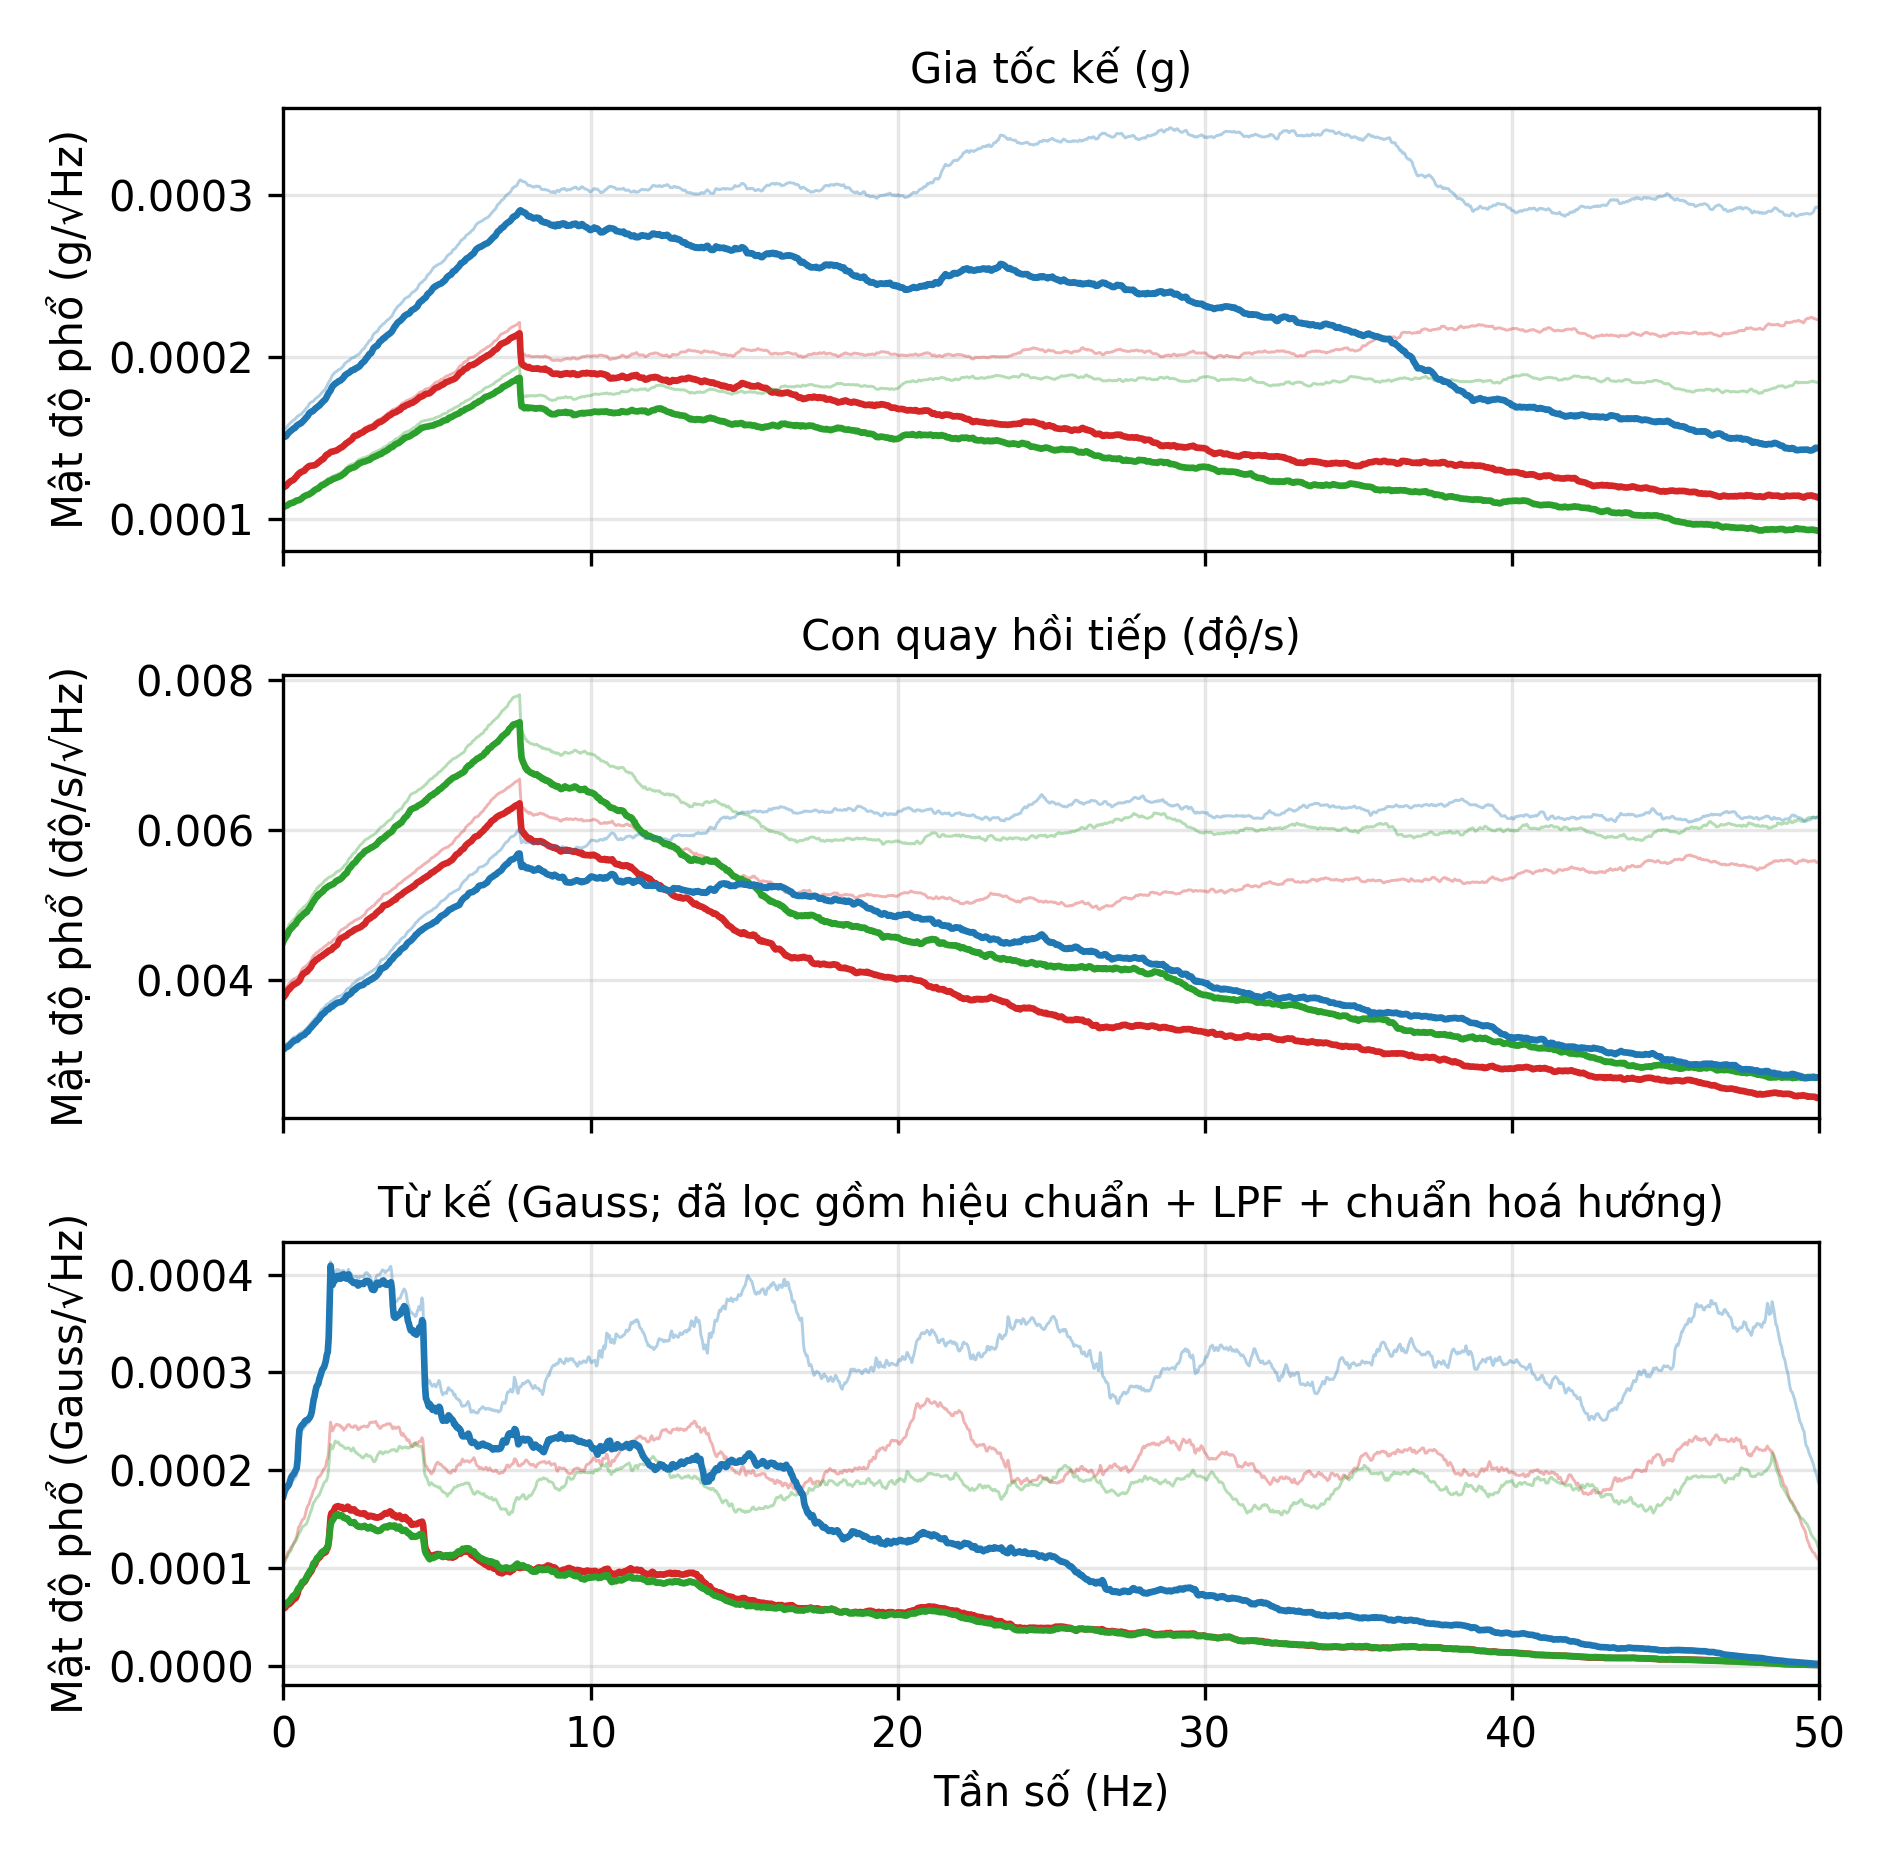
\includegraphics[width=0.9\textwidth]{imgs/fig5_fft_raw_filt.png}
\caption{Phổ nhiễu thô (đường mảnh) và đã lọc (đường đậm) của ba cảm biến trên cùng trục tần số; màu đỏ, xanh lá, xanh dương lần lượt là trục X, Y, Z. Điểm gãy của đường đậm đúng tại tần số cắt của bộ lọc: khoảng 8~Hz với con quay, 30~Hz với gia tốc kế, 10~Hz với từ kế. Phổ từ kế đã lọc được nhân với cường độ từ trường trung bình đo được để đưa về cùng thang Gauss -- luồng này đã qua hiệu chuẩn, lọc và chuẩn hoá hướng nên bản chất so sánh là về hình dạng phổ.}\label{fig:kq-fft}
\end{figure}

Ba điểm gãy trong hình~\ref{fig:kq-fft} khớp đúng thiết kế của các bộ lọc thông thấp (đã trình bày ở mục~\ref{sec:ekf-calib}): phía trên tần số cắt, mật độ phổ của luồng đã lọc giảm rõ rệt so với luồng thô. Bảng~\ref{tab:kq-noise} lượng hoá tác dụng này bằng độ lệch chuẩn $\sigma$ -- độ phân tán của số đo quanh giá trị trung bình, càng nhỏ càng sạch.

\begin{table}[h]
\centering
\caption{Độ lệch chuẩn nhiễu của từng luồng cảm biến (bệ thử tĩnh, phiên LOG\_0032)}
\label{tab:kq-noise}
\begin{tabular}{p{3.1cm}p{1.9cm}p{3.2cm}p{3.4cm}p{2.2cm}}
\toprule
Luồng & Đơn vị & $\sigma$ thô & $\sigma$ đã lọc & Giảm nhiễu \\
\midrule
Gia tốc kế & g & 0,0049--0,0056 & 0,0022--0,0036 & 1,5--2,5 lần \\
Con quay & độ/s & 0,131--0,220 & 0,051--0,180 & 1,2--2,6 lần \\
Từ kế & Gauss & 0,0016--0,0030 & ---\textsuperscript{a} & ---\textsuperscript{a} \\
Áp suất & Pa & 4,04 & ---\textsuperscript{b} & ---\textsuperscript{b} \\
\bottomrule
\end{tabular}

{\footnotesize
\textsuperscript{a}~Luồng từ kế đã lọc được chuẩn hoá về độ dài đơn vị nên khác thang đo, không so sánh trực tiếp được; nhiễu từ kế được xử lý bằng hiệu chuẩn và bộ lọc Kalman (chương~4). \
\textsuperscript{b}~Áp suất không có luồng lọc riêng; việc làm mượt do chính bộ lọc độ cao đảm nhiệm (mục~\ref{sec:kq-ekf}).}
\end{table}

Ngoài độ sạch tín hiệu, chuỗi đo cũng cho biết các luồng dữ liệu đến đều đặn đến mức nào. Bảng~\ref{tab:kq-streamjit} thống kê chu kỳ lấy mẫu đo được từ dấu thời gian trong bản ghi: sai lệch so với tần số danh định dưới 0,2\% với con quay/gia tốc kế và từ kế; riêng áp suất có chu kỳ thỉnh thoảng gấp đôi (tần số đo 49,0~Hz thay vì 50~Hz), phù hợp với đặc tính của BMP180: mỗi lần đo cần tới 13,5~ms trên đường truyền dữ liệu chia sẻ với từ kế.

\begin{table}[h]
\centering
\caption{Đều đặn của các luồng dữ liệu cảm biến (đo từ dấu thời gian của bản ghi)}
\label{tab:kq-streamjit}
\setlength{\tabcolsep}{4pt}
\begin{tabular}{p{3.4cm}p{2.4cm}p{2.6cm}p{2.8cm}}
\toprule
Luồng & Tần số danh định (Hz) & Tần số đo được (Hz) & Độ lệch chu kỳ $\sigma$ ($\mu$s) \\
\midrule
Con quay, gia tốc kế & 500 & 500,00 & 55--57 \\
Từ kế & 100 & 100,00 & 72 \\
Áp suất & 50 & 49,04 & 2\,766 \\
\bottomrule
\end{tabular}
\end{table}

\section{Khối ước lượng hoạt động trên phần cứng}\label{sec:kq-ekf}

Khối ước lượng gồm bộ lọc Kalman mở rộng (EKF -- thuật toán hợp nhất dữ liệu nhiều cảm biến, đã trình bày chi tiết ở chương~4) tư thế bảy trạng thái và bộ lọc độ cao ba trạng thái. Phần này kiểm chứng trên phần cứng thật: nguồn dữ liệu đầu vào của bộ lọc độ cao, và đầu ra của cả hai bộ lọc.

Trước hết, nhiễu của nguồn đo độ cao -- cảm biến áp suất -- được lượng hoá trong hình~\ref{fig:kq-baro}: trên bệ tĩnh, độ cao quy đổi từ áp suất dao động với độ lệch chuẩn 0,34~m (tương đương 4,0~Pa). Đây chính là căn cứ chọn hiệp phương sai đo lường $R = 17{,}8$~Pa\textsuperscript{2} của bộ lọc độ cao: thông số được đặt xấp xỉ phương sai nhiễu đo được thực tế, thay vì chọn cảm tính. Bộ lọc độ cao kết hợp dự báo từ gia tốc kế với phép đo áp suất này, nhờ đó làm mượt dao động nhiễu của áp suất~\cite{sabatini2014}.

\begin{figure}[h]
\centering
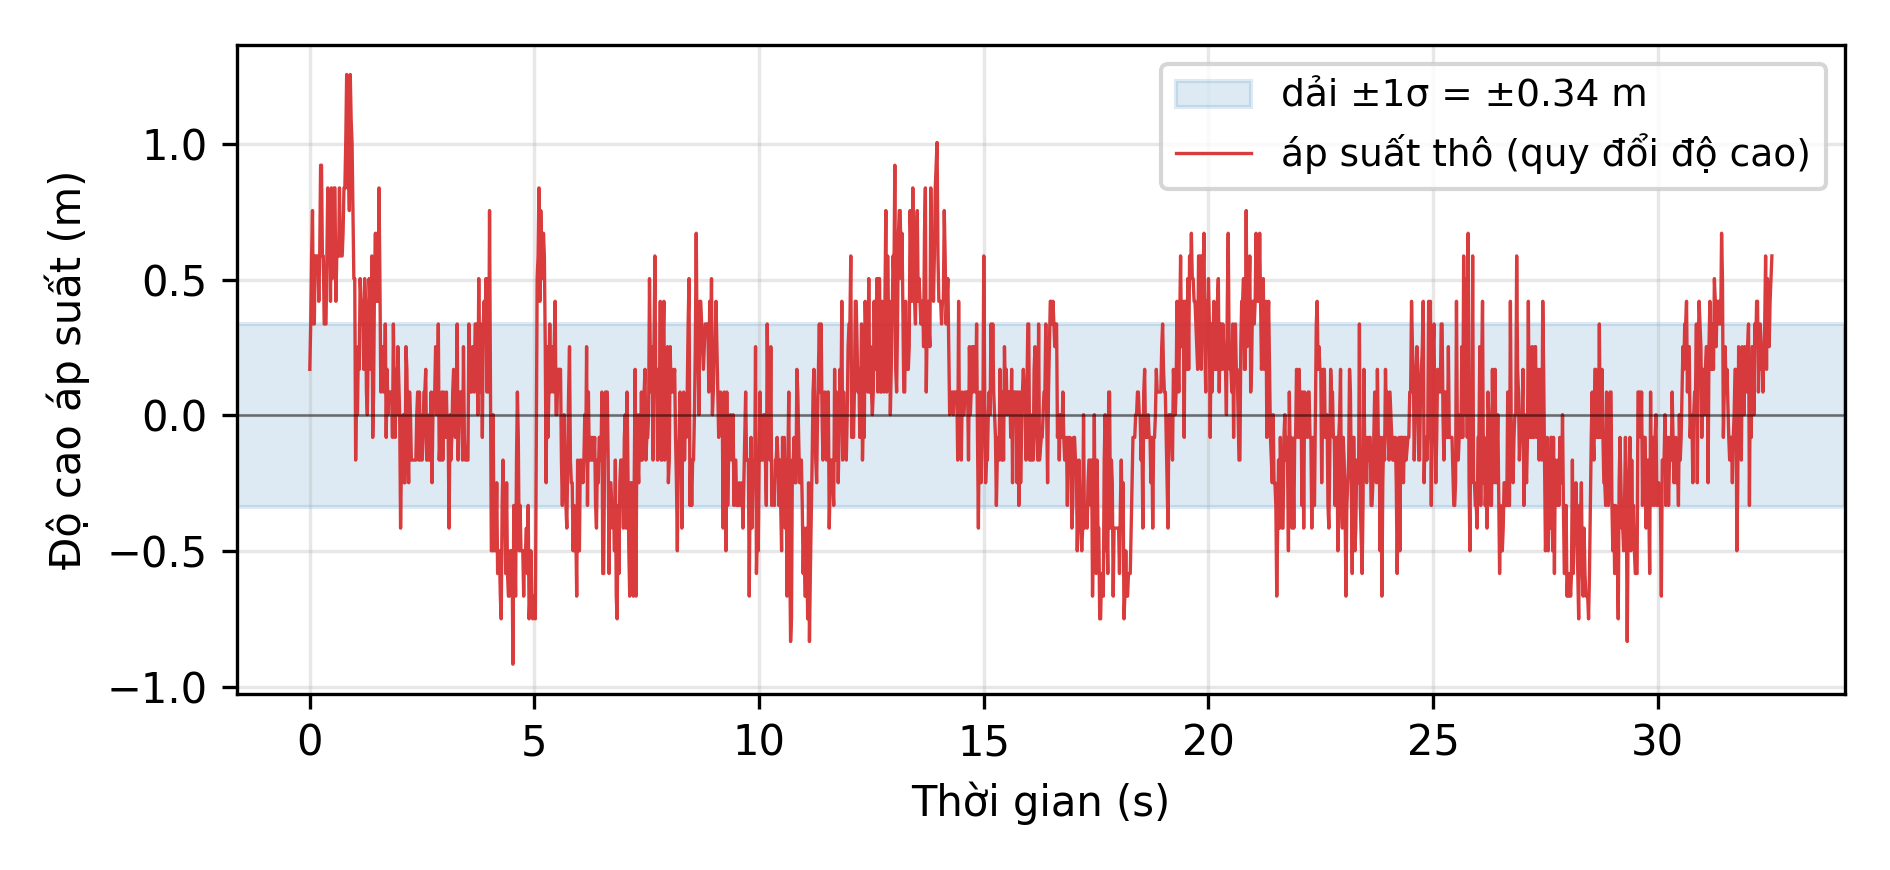
\includegraphics[width=0.9\textwidth]{imgs/fig5_baro_noise.png}
\caption{Độ cao quy đổi từ áp suất trên bệ thử tĩnh (phiên LOG\_0032, đã bỏ giá trị trung bình). Dải xanh là dải $\pm1\sigma = \pm0{,}34$~m của nhiễu áp suất -- nguồn nhiễu mà bộ lọc độ cao phải xử lý.}
\label{fig:kq-baro}
\end{figure}

Đầu ra của cả hai bộ lọc được minh hoạ trong hình~\ref{fig:kq-att}, thu từ phiên blackbox bật luồng tư thế và độ cao (phiên LOG\_0037, 27,5~giây thao tác tay trên bệ thử). Về bộ lọc tư thế: các góc roll/pitch bám theo động thái xoay tay với biên độ tới $\pm55$\textdegree{}; góc yaw quay trọn vòng. Các nhảy đột ngột giữa $+180$\textdegree{} và $-180$\textdegree{} là cách biểu diễn chuẩn của phép quy đổi góc, không phải lỗi ước lượng.

\begin{figure}[h]
\centering
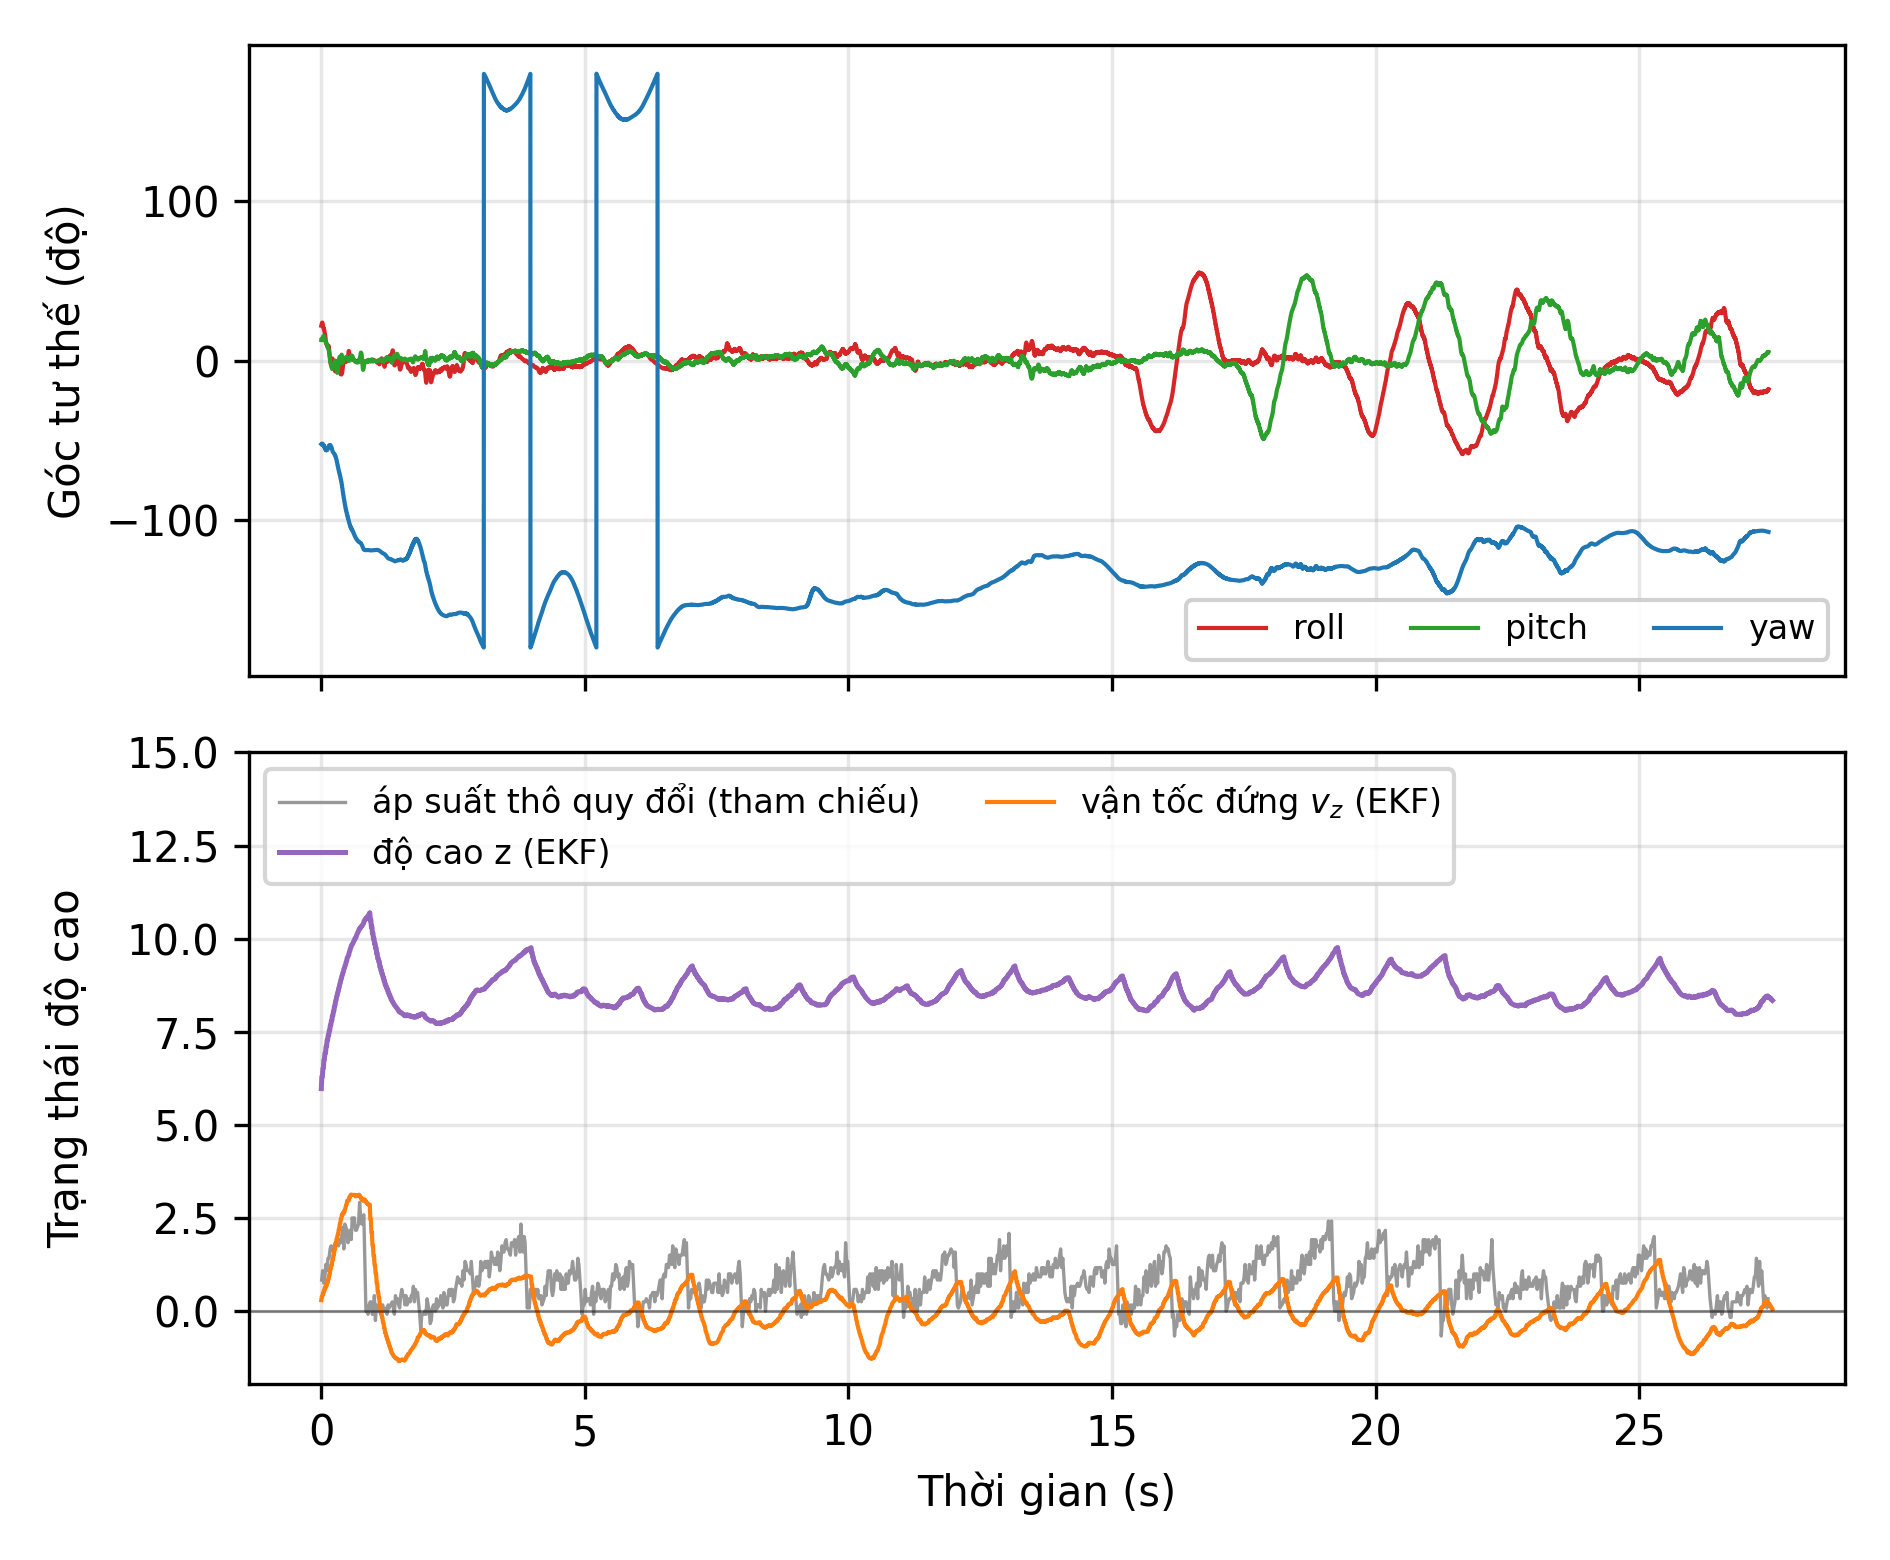
\includegraphics[width=0.87\textwidth]{imgs/fig5_ekf_output.png}
\caption{Đầu ra của hai bộ lọc EKF khi thao tác tay trên bệ thử (phiên LOG\_0037, 27,5~giây). Trên: góc roll/pitch/yaw do EKF tư thế đưa ra. Dưới: độ cao $z$ và vận tốc đứng $v_z$ của EKF độ cao, kèm đường tham chiếu quy đổi từ áp suất thô.}
\label{fig:kq-att}
\end{figure}

Về bộ lọc độ cao: trạng thái $z$ dao động trong vùng 6--10,7~m suốt cửa sổ ghi -- ngay từ mẫu đầu, $z$ đã ở mức 6,0~m, tức phần lệch nền hình thành trước hoặc ngay đầu lúc ghi, do tích phân gia tốc bị sai khi phép chiếu lệch trong lúc xoay và chưa được áp suất kéo về trong thời gian ghi. Dao động ngắn hạn của $z$ theo kịp một phần đường tham chiếu áp suất (biên độ ~3,6~m), phần nền còn lại là trôi của tích phân. Đây là hạn chế đã biết của bộ lọc độ cao khi chưa có cảm biến quang học phụ trợ, được ghi nhận trong hướng phát triển ở chương~6.

\section{Hiệu năng thời gian thực của bộ định thời}\label{sec:kq-rtos}

Yêu cầu cốt lõi của bộ điều khiển bay là mọi tác vụ chạy đúng chu kỳ. Phần mềm đo yêu cầu này bằng bộ ghi định thời tích hợp sẵn: mỗi khi một tác vụ hoàn thành một vòng làm việc, hệ thống ghi một bản ghi 12~byte gồm thời điểm bắt đầu, thời điểm kết thúc, mã tác vụ và nhân xử lý. Bản ghi được ghi vào bộ đệm 4~MB trên PSRAM (bộ nhớ ngoài của vi điều khiển), sau đó được bơm xuống thẻ SD theo từng khối. Bộ ghi tự khởi động sau 3~giây kể từ lúc bật nguồn, ghi liên tục 20~giây, bao phủ toàn bộ 19 tác vụ.

Từ bản ghi này, chương trình phân tích rút ra cho từng tác vụ: tần số đo được so với tần số thiết kế, độ lệch chu kỳ (jitter -- mức dao động của chu kỳ quanh giá trị danh nghĩa), thời gian chạy trung bình và thời gian chạy dài nhất quan sát được (WCET), tỷ lệ sử dụng hai nhân xử lý và số lần tác vụ di chuyển giữa hai nhân.

Kết quả dưới đây lấy từ một bản ghi thật (phiên TRC\_0008): cửa sổ 20~giây, 47~216 bản ghi, không mất bản ghi nào; bộ kiểm định tính toàn vẹn của chương trình phân tích đánh giá đạt (đuôi tệp nằm đúng vị trí, không có bản ghi hỏng, số vòng lặp của mỗi tác vụ khớp tần số danh định). Bảng~\ref{tab:kq-trace} tổng hợp số liệu của 12 tác vụ định kỳ có hoạt động trong cửa sổ ghi; các tác vụ theo yêu cầu (bốn tác vụ hiệu chuẩn, OTA) và tác vụ LED theo sự kiện không có vòng lặp trong 20~giây nên không xuất hiện.

\begin{table}[h]
\centering
\footnotesize
\setlength{\tabcolsep}{3pt}
\caption{Số liệu định thời đo được của 12 tác vụ định kỳ (bệ thử tĩnh, phiên TRC\_0008, 20~giây)}
\label{tab:kq-trace}
\begin{tabular}{lp{1.5cm}p{1.7cm}p{1.4cm}p{1.5cm}p{1.5cm}p{1.4cm}}
\toprule
Tác vụ & Tần số đo (Hz) & Chu kỳ TB ($\mu$s) & p99 ($\mu$s) & Jitter $\sigma$ ($\mu$s) & Chạy TB ($\mu$s) & WCET ($\mu$s) \\
\midrule
ACCEL\_GYRO\_DAQ & 500,01 & 2\,000,0 & 2\,377 & 163,9 & 1\,045,3 & 2\,177 \\
ACCEL\_GYRO\_PREPROCESS & 499,99 & 2\,000,0 & 2\,292 & 113,1 & 39,4 & 733 \\
EKF\_ROLL\_PITCH & 500,00 & 2\,000,0 & 2\,244 & 115,3 & 369,7 & 764 \\
MOTOR & 250,00 & 4\,000,0 & 4\,038 & 25,8 & 21,2 & 157 \\
MAG\_DAQ & 100,00 & 9\,999,9 & 10\,317 & 199,2 & 1\,918,3 & 2\,987 \\
MAG\_PREPROCESS & 100,00 & 9\,999,9 & 10\,256 & 163,5 & 48,7 & 510 \\
FSM\_MAIN & 100,00 & 10\,000,0 & 10\,129 & 104,1 & 31,4 & 774 \\
EKF\_ALTITUDE & 100,00 & 9\,999,9 & 10\,337 & 208,0 & 134,8 & 579 \\
EKF\_YAW & 99,50 & 10\,050,3 & 10\,273 & 703,0 & 227,4 & 463 \\
BARO\_DAQ & 50,00 & 20\,000,0 & 20\,132 & 39,7 & 1\,011,4 & 2\,776 \\
RC\_RECEIVER & 50,00 & 20\,000,0 & 20\,003 & 12,2 & 5\,579,1 & 5\,818 \\
SD\_LOGGER & 10,00 & 99\,953,4 & 100\,117 & 1\,636,9 & 5\,964,5 & 114\,837 \\
\bottomrule
\end{tabular}

{\footnotesize
Trong bản build bệ thử, SD\_LOGGER đảm nhiệm vai trò bơm dữ liệu trace xuống thẻ (10~Hz, ưu tiên thấp nhất, tách khỏi đường điều khiển). EKF\_YAW đo được 99,50~Hz -- thiếu 9 vòng lặp trong cửa sổ ghi, hiện tượng đang được theo dõi. Máy thu điều khiển RC\_RECEIVER là tác vụ duy nhất dịch chuyển giữa hai nhân xử lý (915 lần trong 20~giây).}
\end{table}

Chuỗi xử lý 500~Hz -- thu dữ liệu, tiền xử lý và dự báo EKF tư thế -- đo được đúng 500,0~Hz trong suốt 20~giây (mỗi tác vụ hoàn thành tròn 10\,000 vòng). Độ lệch chu kỳ của cả ba tác vụ này chỉ 113--164~$\mu$s, tương đương 6--8\% chu kỳ; thời gian chạy dài nhất quan sát được của tác vụ nặng nhất (EKF tư thế) là 764~$\mu$s, chiếm 38\% ngân sách 2~ms~\cite{cervin2003}. Tất cả các tác vụ định kỳ khác đều có thời gian chạy dài nhất dưới 30\% chu kỳ của chúng. Hình~\ref{fig:kq-trace-hist} cho thấy phân bố chu kỳ của sáu tác vụ tiêu biểu: hầu hết các vòng lặp dồn quanh giá trị danh nghĩa, những vòng lệch xa chỉ chiếm phần trăm nhỏ và không có xu hướng trôi dần.

\begin{figure}[h]
\centering
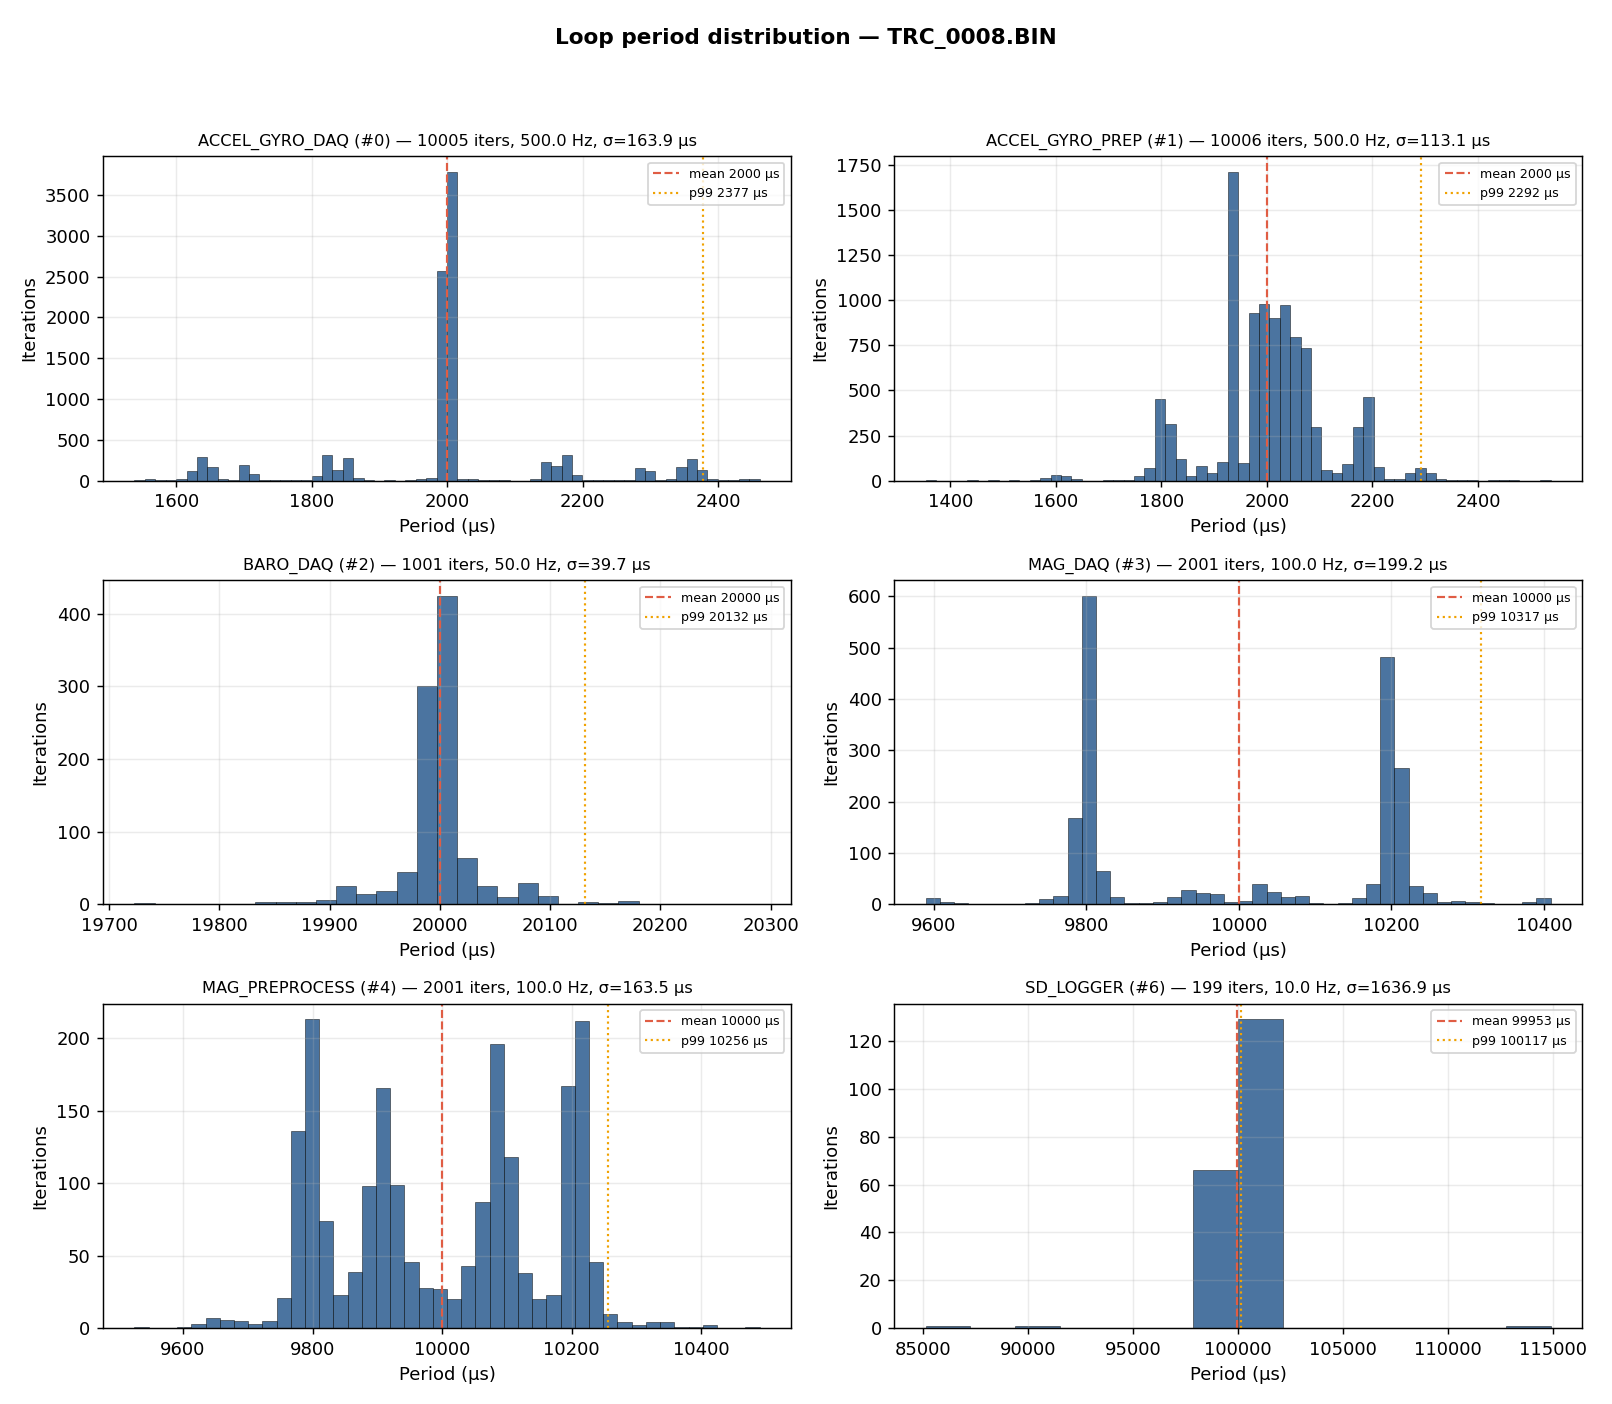
\includegraphics[width=0.84\textwidth]{imgs/fig5_trace_period_hist.png}
\caption{Phân bố chu kỳ của sáu tác vụ tiêu biểu trong cửa sổ ghi 20~giây (phiên TRC\_0008). Đường đứt nét đỏ: chu kỳ trung bình; đường chấm vàng: mốc p99. Tác vụ thu dữ liệu 500~Hz dồn quanh đúng 2\,000~$\mu$s; các phân bố lệch nhẹ do thứ tự được lập lịch, nhưng p99 vẫn trong vài trăm $\mu$s so với danh nghĩa.}
\label{fig:kq-trace-hist}
\end{figure}

\section{Nhận xét tổng hợp}\label{sec:kq-tonghop}

Trên bệ thử tĩnh, các kết quả kiểm chứng đạt được như sau. Chuỗi thu dữ liệu cảm biến chạy đúng tần số thiết kế 500, 100 và 50~Hz, lệch dưới 0,2\% (trừ áp suất 49,0~Hz do đặc tính của BMP180). Bộ lọc thông thấp phát huy đúng tác dụng thiết kế: giảm nhiễu con quay 1,2--2,6 lần và gia tốc kế 1,5--2,5 lần. Nhiễu nguồn đo độ cao đã được lượng hoá (0,34~m) và là căn cứ chọn thông số của bộ lọc độ cao. Hệ thống tự kiểm tra năm cổng trước mỗi phiên đo hoạt động đầy đủ; hai công cụ ghi dữ liệu (blackbox và trace) chạy ổn định trên phần cứng. Bộ định thời chạy đúng chu kỳ trên toàn bộ tác vụ định kỳ: chuỗi 500~Hz bám sát mục tiêu với độ lệch chu kỳ 6--8\% chu kỳ, và thời gian chạy dài nhất của tác vụ nặng nhất chỉ chiếm 38\% ngân sách thời gian của nó; bộ ghi trace thu 47~216 bản ghi trong 20~giây không mất một bản ghi nào.

Các hạn chế hiện tại thuộc hai loại. Thứ nhất, mọi số liệu thu trên bệ tĩnh, chưa phản ánh rung động động cơ và điều kiện khi bay thật -- phân tích phổ ở chế độ bay là việc kế tiếp. Thứ hai, chất lượng cảm biến áp suất còn hạn chế: nhiễu 0,34~m và các chu kỳ đo bị bỏ sót là giới hạn phần cứng của BMP180; hướng nâng cấp cảm biến và các hướng phát triển tiếp theo được trình bày ở chương~6.
